\documentclass[fleqn,11pt]{paper}

%% This is the Homework LaTeX template.  Use this file to fill in your solutions. 
%%
%% Notes: 
%%    1. If possibly, try to write your answers inside a \begin{solution}...\end{solution}
%%    environment.
%%
%%    2. If you enter your answers into this Homework*.tex source file, you
%%    will have to compile it into a pdf document.  There are a number of ways to
%%    do that. Probably the easiest is to use the website called ShareLaTeX.com.
%%    Alternatively,
%%
%%       Mac OS X users: you might try MacTeX. 
%%       Linux users: most come with TeX; otherwise do a full install of TeXLive.
%%       Windows users: ...proTeXt maybe? (or switch to a better operating system) 
%%
%%       There is a Makefile in this directory, so (on Linux) you could just 
%%       enter `make` to compile all the Homework*.tex files at once (assuming
%%       you have everything set up properly).
%%
%%    3. Please don't hesitate to inform the professor if you have trouble, or open
%%       a ``New issue'' on GitHub or post to Piazza or ask in lecture.
%%
%%    4. Update the title and date if necessary.
         \title{Math 317: Computer Lab 1}
         \date{Due: 29 January 2016, 2pm}


%%%%%%%%%%%%%%%%%%%%%%%%%%%%%%%%%%%%%%%%
% Basic packages
%%%%%%%%%%%%%%%%%%%%%%%%%%%%%%%%%%%%%%%%
\usepackage[letterpaper,top=3cm,bottom=3cm,left=2.5cm,right=2.5cm]{geometry}
\usepackage{tikz-cd}
\usepackage{scalefnt}
\usepackage{amsmath,amsthm,amssymb}
\usepackage{mathtools}
\usepackage{etoolbox}
\usepackage{fancyhdr}
\usepackage{xcolor}
\usepackage[colorlinks=true,urlcolor=blue,linkcolor=blue,citecolor=blue]{hyperref}
\usepackage{xspace}
\usepackage{comment}
\usepackage{url} % for url in bib entries
\usepackage{mathrsfs}

\theoremstyle{remark}
\newtheorem{theorem}{Theorem}
\newtheorem{exercise}{Exercise}
\newtheorem*{prop}{Proposition}
\newtheorem{problem}{Problem}
\newtheorem*{prob}{Problem}
\newtheorem*{solution}{{\bf Solution}}
\newtheorem*{hint}{{\it Hint}}
\newtheorem*{ex}{Exercise}


%%%%%%%%%%%%%%%%%%%%%%%%%%%%%%%%%%%%%%%%%%%%%%%%%%
%% Surround the problem and solution with 
%% \begin{ProbBox}  and   \end{ProbBox}
%% to prevent pagebreaks.
\newenvironment{ProbBox}{\noindent\begin{minipage}{\linewidth}}{\end{minipage}}

%%%%%%%%%%%%%%%%%%%%%%%%
% Fancy page style     %
%%%%%%%%%%%%%%%%%%%%%%%%
\pagestyle{fancy}
\newcommand{\metadata}[2]{
  \lhead{}
  \chead{}
  \rhead{\bfseries Math 317: Linear Algebra}
  \lfoot{#1}
  \cfoot{#2}
  \rfoot{\thepage}
}
\renewcommand{\headrulewidth}{0.4pt}
\renewcommand{\footrulewidth}{0.4pt}


%%%%%%%%%%%%%%%%%%%%%%%%%%%%%%%%%%
% Customize list enviroonments   %
%%%%%%%%%%%%%%%%%%%%%%%%%%%%%%%%%%
% package to customize three basic list environments: enumerate, itemize and description.
%% \usepackage{enumitem}
%% \setitemize{noitemsep, topsep=0pt, leftmargin=*}
%% \setenumerate{noitemsep, topsep=0pt, leftmargin=*}
%% \setdescription{noitemsep, topsep=0pt, leftmargin=*}

\usepackage{enumerate}

%%%%%%%%%%%%%%%%%%%%%%%%%%%%
%% Space between problems  %
%%%%%%%%%%%%%%%%%%%%%%%%%%%%
\newrobustcmd*{\probskip}{\vskip1cm}

%%    Try to use standard notation, as used in class and in the textbook.
%%    For the most basic symbols, you may wish to use LaTeX macros to keep 
%%    the conventions you use consistent and easy to remember.

%%%%%%%%%%%%%%%%%%%%%%%%%%
%%    Math shortcuts     %
%%%%%%%%%%%%%%%%%%%%%%%%%%
\newcommand\join{\ensuremath{\vee}}
\newcommand\meet{\ensuremath{\wedge}}
\newcommand\R{\fld{R}}
\newcommand\proj{\ensuremath{\operatorname{proj}}}
\newcommand\End{\ensuremath{\operatorname{End}}}
\newcommand\Aut{\ensuremath{\operatorname{Aut}}}
\newcommand\Hom{\ensuremath{\operatorname{Hom}}}
\newcommand{\Aff}{\ensuremath{\operatorname{Aff}}}
\newcommand{\ann}[1]{\ensuremath{\operatorname{ann}(#1)}}
\newcommand{\id}{\ensuremath{\operatorname{id}}}
\newcommand{\nulity}[1]{\ensuremath{\operatorname{null}(#1)}}
\renewcommand{\ker}[1]{\ensuremath{\operatorname{ker}(#1)}}
\renewcommand{\dim}[1]{\ensuremath{\operatorname{dim}(#1)}}
\newcommand\im[1]{\ensuremath{\operatorname{im}(#1)}}
\newcommand{\rank}[1]{\ensuremath{\operatorname{rank}(#1)}}
\newcommand{\trace}[1]{\ensuremath{\operatorname{trace}(#1)}}
\renewcommand{\phi}{\ensuremath{\varphi}}

\renewcommand{\vec}[1]{\mathbf{#1}}
         \newcommand\alg[1]{\ensuremath{\mathbf{#1}}}
         \newcommand{\<}{\ensuremath{\langle}}
         \renewcommand{\>}{\ensuremath{\rangle}}
         \newcommand\fld[1]{\ensuremath{\mathbb{#1}}}

%%       To make a boldface vector, use backslash v in front of the 
%        letter and add a new command for that letter here.
         \newcommand\va{\vec{a}}
         \newcommand\vb{\vec{b}}
         \newcommand\vu{\vec{u}}
         \newcommand\vv{\vec{v}}
         \newcommand\vw{\vec{w}}
         \newcommand\vx{\vec{x}}
         \newcommand\vy{\vec{y}}
         \newcommand\vz{\vec{z}}
         \newcommand\vzero{\vec{0}}

         \newcommand\sP{\ensuremath{\mathscr P}}
         \newcommand\Span{\ensuremath{\operatorname{Span}}}

%% ---for augmented matrices---
\newenvironment{amatrix}[1]{%
  \left[\begin{array}{@{}*{#1}{r}|rr@{}}
}{%
  \end{array}\right]
}
\newenvironment{amatrix2}[1]{%
  \left[\begin{array}{@{}*{#1}{r}|rr@{}}
}{%
  \end{array}\right]
}

\begin{document}

%%    INSERT YOUR NAME HERE!!!
         \metadata{Name:}{Lab 1 (due 1/29 2pm)}
         \author{NAME:}
%%       Example:
%%         \metadata{Name: William DeMeo}{Lab 1 (due: 2016/01/29 by end of lab)}
%%         \author{NAME: William DeMeo}
%%

\maketitle


%%%%%%%%%%%%%%%%%%%%%%%%%%%%%%%%%%%%%%%%%%%%%%%%%%%%%%%%%

\noindent {\bf Instructions.}
\begin{itemize}
\item This assignment must be completed in the Carver 449 computer lab by 2pm on
  \begin{quote}
    {\bf Friday January 29.}  
  \end{quote}
  Late submissions will not be accepted.
\item {\bf Part 1.} Sign up for an account on the Math Department Sage server and then demonstrate 
  that you know how to compute $2\times 2$ (more detailed instructions are
  below; see Part 1). \\
  Have the instructor sign your paper to record completion of Part 1. 

  Completing Part 1 is worth 1 point. If you are not interested in completing Part 2 of the
  assignment, you may turn in your paper and leave the lab after completing Part 1. \\
  {\bf Make sure your name is on your paper and it was signed by the instructor.}
\item {\bf Part 2.} Complete the exercises in Part 2 following the instructions provided below, 
  then save your Sage worksheet as a .sws file and upload this file on Blackboard.

\item When you have finished working or it is 2pm (whichever comes first): 
  \begin{enumerate}
  \item {\bf stop your Sage worksheet} (Action $\rightarrow$ Save and quit worksheet; or use Stop button),
  \item {\bf sign out of Sage}, 
  \item {\bf logout of your computer}, 
  \item {\bf write your name on your paper},
  \item {\bf hand it in to the instructor}.
  \end{enumerate}
\end{itemize}


%--  Part 1  ---------------------------------------------------
\section*{Part 1}
~
  \begin{enumerate}
  \item Login to any machine in Carver 449, open up a browser (preferably Chrome) and navigate to

    \begin{quote}
      \url{https://sage.math.iastate.edu/}
    \end{quote}

%\hfill    (continued on reverse $\rightarrow$)

\newpage
    You should arrive at a page that looks like this:

    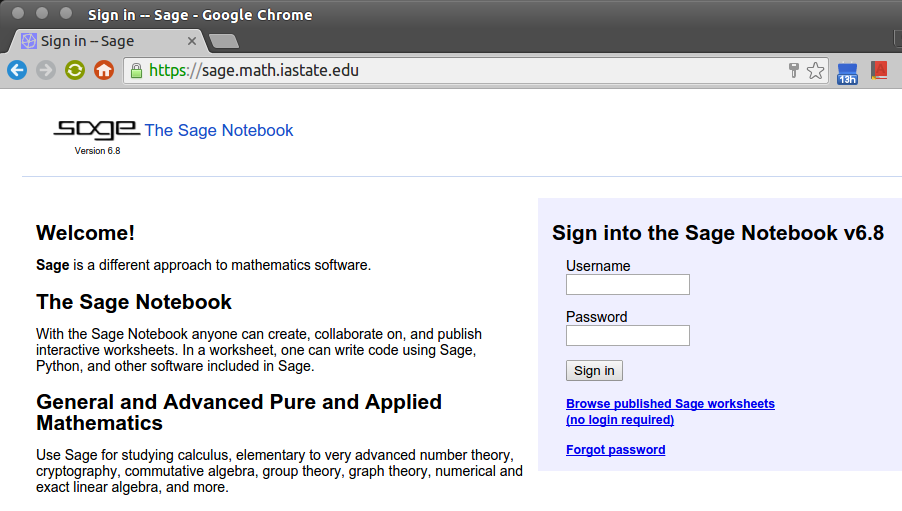
\includegraphics[scale=.4]{Sage-login.png}

  \item Using your Iowa State username and a password supplied by your instructor, login to your
    Sage account.  \\

  \item Once you are logged in, select the New Worksheet link and name the worksheet Lab1.  

    If all went well, you will now see a page that looks like this:

    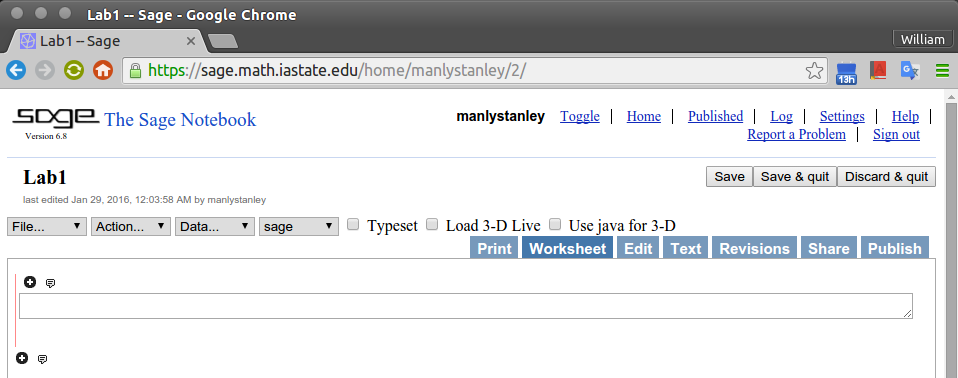
\includegraphics[scale=.4]{Lab1-screen.png}
\\
  \item Click somewhere inside the wide rectangular box (or ``cell'') and type the expression 2*2.
    Then type Shift+Enter (hold down the Shift key and press Enter; or simply click `evaluate`).

    If a 4 appears in the worksheet, congratulations on completing Part 1. Ask the
    instructor to check your work and sign below, then do Part 2 (or Save \& quit if you want to stop here):\\
    \\\\
    Instructor signature: \underline{\phantom{XXXXXXXXXXXXXXXXXXXXXXXXXXXXXXXX}} (1 point)

  \end{enumerate}

\newpage
%--  Part 2  ---------------------------------------------------
\section*{Part 2}
In this part we will use Sage to help solve the following exercise from the textbook:
\begin{quote}
%--  PROBLEM 1  ---------------------------------------------------
\begin{prob}[SA 1.5.1]
  By solving a system of equations, write the vector
  \[
  \vb = \begin{bmatrix*}[r] 3 \\ 0 \\ -2 \end{bmatrix*}
  \; \text{ as a linear combination of the vectors } \;
  \vv_1 = \begin{bmatrix*}[r] 1 \\ 0 \\ -1 \end{bmatrix*},
  \;
  \vv_2 = \begin{bmatrix*}[r] 0 \\ 1 \\ 2 \end{bmatrix*},
  \; \text{ and } \;
  \vv_3 = \begin{bmatrix*}[r] 2 \\ 1 \\ 1 \end{bmatrix*}.
  \]
\end{prob}
\end{quote}

\vskip1cm
\begin{solution}
  To write the vector $\vb$ as a linear combination of the vectors
  $\vv_1$, $\vv_2$,  and $\vv_3$, we must find coefficients 
  $x_1, x_2, x_3$ such that $\vb = x_1 \vv_1 +  x_2 \vv_2 + x_3 \vv_3$.  
  As we discussed in lecture, this is equivalent to
  finding a vector $\vx = (x_1, x_2, x_3)$ such that $A\vx = \vb$, where $A$ is
  the matrix whose columns are the vectors $\vv_1$, $\vv_2$, and $\vv_3$.  

  In Sage, we will construct the matrix $A$ and then augment this matrix with the 
  vector $\vb$. Finally we will solve for $\vx$ by putting the augmented matrix 
  in echelon form. We'll make Sage do all the tedious work, but it will be 
  up to us to interpret Sage's output and write down a correct solution.
  
\end{solution}
  
  \begin{enumerate}
  \item First, we need to learn how to enter the matrix
    \[
    A = \begin{bmatrix*}[r] 1 &0&2\\ 0&1&1\\-1&2&1\end{bmatrix*} %, \; 
      %% \vb = \begin{bmatrix*}[r] 3 \\ 0 \\ -2 \end{bmatrix*}
      \]
      in Sage.
      In your Lab1 Sage worksheet, click the {\bf Help} link at the top right.  A help
    window should appear (possibly in a pop-up window). On the Help page, navigate through the following links: 
    \begin{quote}
    {\bf Reference Manual} $\rightarrow$ {\bf modules} $\rightarrow$ {\bf m} $\rightarrow$ {\bf sage.matrix.constructor}
    \end{quote}
    From the help page that appears, you should be able to discern how to input the matrix $A$ in
    Sage. (Hint: you should start with {\tt A = matrix([[1,0,2],[}...)

    After entering the matrix, type Shift+Enter to evaluate your input.  
    To confirm that Sage correctly interpreted your
    input, enter the single character {\tt A} in a new cell and then Shift+Enter.
  \item Next, input the vector $\vb = (3, 0, -2)$ using the following syntax:
    \begin{verbatim}
     b = vector([3,0,-2])
    \end{verbatim}
    At this point, you are half way done with Part 2.  Ask the instructor to check your work.\\
    \\\\
    Instructor signature: \underline{\phantom{XXXXXXXXXXXXXXXXXXXXXXXXXXXXXXXX}} (1/2 point)
\newpage


  \item Next, we want to construct the augmented matrix 
    \[
      [A|\vb] = 
      \begin{amatrix}{3} 
        1 &0&2&3\\ 0&1&1&0\\-1&2&1&-2
      \end{amatrix}.
      \]
      Using a search engine (e.g., Google) search for the phrase ``sage augmented matrix.''  The
      first result will probably be to the Sage Reference Manual page
      {\tt matrices/sage/matrix/matrix1.html}.  

      Read a bit of this page and see if you can 
      figure out how to use the {\tt augment()} function (or \emph{method}) of the matrix 
      object {\tt A}.
      You will use {\tt b} as the input to the  {\tt augment()} method.
      
      Don't forget to give a name to the augmented matrix, e.g., {\tt Ab = augment}... and then
      check that Sage correctly interpreted your input (by typing {\tt Ab} then Shift+Enter.)

    \item Next, put your augmented matrix in echelon form.  Again, try to use the Sage help pages
      or a Google search to figure out how to do this.  If you need help, ask the instructor.

    \item Finally, interpret the Sage output of the {\tt echelon\_form} command and write down a
      solution.
      
      The solution vector is 
\vskip5mm
\[\vx = \]
\vskip1cm
      ...so $\vb = (3, 0, -2)$ can be written as the following linear combination: 
\vskip5mm
\[
\vb = \text{\underline{\phantom{XXX}}}\vv_1 + \text{\underline{\phantom{XXX}}} \vv_2+
\text{\underline{\phantom{XXX}}} \vv_3.
\]
\vskip5mm
%% This shows that the vector $\vx = (1, -1, 1)$ solves $A\vx = \vb$.  To check this,
You have now completed Part 2.  By the way, you can also use Sage to check your final 
answer. One way to do this is to type your solution vector  
into Sage (with {\tt x = vector([}...) and then compute {\tt A*x}.  Does this result in the vector $(3, 0, -2)$?
Alternatively, you could simply ask Sage to solve the system for you with %% {\tt A.solve\_right(b)}!
the {\tt solve\_right} command!
  \end{enumerate}
\vskip5mm
\noindent A tutorial describing how to do more linear algebra in Sage is available at
\begin{quote}
\url{http://doc.sagemath.org/html/en/tutorial/tour_linalg.html}
\end{quote}
\vskip 1cm
    Instructor signature: \underline{\phantom{XXXXXXXXXXXXXXXXXXXXXXXXXXXXXXXX}} (1/2 point)

\end{document}

  \end{enumerate}
\end{Solution}

%%  PAGE 4  %%%%%%%%%%%%%%%%%%%%%%%%%%%%%%%%%%%%%%%%%%%%%%%%%%%%%%%

%% \bibliographystyle{plain}
%% \bibliography{refs}

\end{document}
